\documentclass[a4,danish]{article}
\usepackage[a4paper, margin=3.5cm]{geometry}
% Standard library
\usepackage[utf8]{inputenc}
\usepackage[T1]{fontenc}
\usepackage{natbib, dsfont, enumitem,
  amssymb,soul,xcolor,amsmath,graphicx,subcaption,verbatim,pgfplots,tikz}
\usetikzlibrary{calc,patterns,angles,quotes,automata, positioning,arrows,shapes}

% Ref and bibliography style 
\bibliographystyle{abbrvnat}

% Handling new lines
\setlength{\parskip}{1em}
\setlength{\parindent}{0em}

% Handling space after sections
\usepackage{titlesec}
\titlespacing*{\section}{0em}{2em}{0em}
\titlespacing*{\subsection}{0em}{2em}{0em}
\titlespacing*{\subsubsection}{0em}{2em}{0em}

% No spacing after in start of list
\setlist[itemize]{topsep=0pt}
\setlist[enumerate]{topsep=0pt}

% Todo and notes
\usepackage[author=]{fixme}
\fxusetheme{color}
\definecolor{fxtarget}{rgb}{1,0.6,0}
\definecolor{fxnote}{rgb}{1,0.6,0}

\newcommand{\darkmode}[1]{ % Set dark mode or not
  \ifthenelse{ \equal{#1}{1}}{
    \usepackage{pagecolor}
    \definecolor{pagecol}{RGB}{0,43,54}
    \definecolor{textcol}{RGB}{131,148,150}
    % \definecolor{textcol}{RGB}{38,139,210}
    \pagecolor{pagecol}
    \color{textcol}
  }
}
% New operators and commands
\newcommand{\Z}{\mathbb{Z}}
\newcommand{\Q}{\mathbb{Q}}
\newcommand{\R}{\mathbb{R}}
\newcommand{\N}{\mathbb{N}}
\newcommand{\C}{\mathbb{C}}
\renewcommand{\S}{\mathbb{S}}
\newcommand{\blank}{\makebox[1ex]{\textbf{$\cdot$}}}
\newcommand\independent{\protect\mathpalette{\protect\independenT}{\perp}}
\def\independenT#1#2{\mathrel{\rlap{$#1#2$}\mkern2mu{#1#2}}}
\renewcommand{\phi}{\varphi}
\renewcommand{\epsilon}{\varepsilon}
\newcommand*\diff{\mathop{}\!\mathrm{d}}
\newcommand{\weakly}{\rightsquigarrow}
\newcommand\smallO{
  \mathchoice
    {{\scriptstyle\mathcal{O}}}% \displaystyle
    {{\scriptstyle\mathcal{O}}}% \textstyle
    {{\scriptscriptstyle\mathcal{O}}}% \scriptstyle
    {\scalebox{.6}{$\scriptscriptstyle\mathcal{O}$}}%\scriptscriptstyle
}
\newcommand{\midd}{\; \middle|\;}
\newcommand{\1}{\mathds{1}}
\usepackage{ifthen} %% Empirical process with default argument
% \newcommand{\G}[1][]{%
%    \ifthenelse{ \equal{#1}{} }
%       {\ensuremath{\mathbb{G}_n}}
%       {\ensuremath{\mathbb{G}_{#1}}}
% }
% New version:
\newcommand{\G}[2][n]{
{\ensuremath{\mathbb{G}_{#1}}{\left[#2\right]}}
}
\DeclareMathOperator*{\argmin}{\arg\!\min}

% New operators for consistent notation
\newcommand{\V}{\mathrm{Var}} % variance
\newcommand{\measure}[1]{\mathrm{{#1}}} % measure
% \newcommand{\measure}[1]{\textnormal{\textbf{{#1}}}} % measure
\newcommand{\m}[1]{\measure{#1}} % measure shortcut
\newcommand{\eqd}{\stackrel{d}{=}} % equality in distribution
\newcommand{\arrowP}{\xrightarrow{\; \m{P} \;}} % convergence in probability
\newcommand{\leb}{\lambda} % the Lebesgue measure
\newcommand{\T}{\top} % transpose

\usepackage{xargs}
% Make it easy to change counterfactual notation:
\newcommandx{\cf}[4][3={}, 4={}]{
  % \ifthenelse{ \equal{#4}{} }
  % {{#1^{#2}}(#3)}
  {\ifthenelse{ \equal{#3}{} }
    {{#1^{#2}}_{#4}}
    {{#1^{#2}}_{#4}(#3)}}
}

% Easily change notation:
\DeclareMathOperator{\TT}{\Psi} % target parameter
\newcommand{\lp}{\mathcal{L}_{\P}^2} % shortcut for lp2 space
\newcommand{\empmeas}{\hat{\mathbb{P}}_n} % empirical measure
\DeclareMathOperator{\E}{\mathbb{E}} % expectation
\renewcommand{\P}{\m{P}} % probability
\newcommand{\ic}{\mathrm{IF}} % influence curve
% Testing!:
% Def, theorems, etc. -- maybe review this
\usepackage{amsthm}

% Style separating env slightly from the rest
\newtheoremstyle{break}  
	{\topsep}{\topsep}
	{}{}
	{\bfseries}{}
	{\newline}{}
% Adjusted thm-environment with bullet at end
\newcommand{\newmarkedtheorem}[1]{%
  \newenvironment{#1}
    {\pushQED{\leavevmode\unskip\penalty9999 \hbox{}\nobreak\hfill
  \quad\hbox{\(\bullet\)}}
    \csname inner@#1\endcsname}
    {\popQED\csname endinner@#1\endcsname}%
  \newtheorem{inner@#1}%
}

\theoremstyle{plain} % plain italic style
\newtheorem{theorem}{Theorem}
\numberwithin{theorem}{section}
\newtheorem*{theorem*}{Theorem}
\newtheorem{conjecture}{Conjecture}
\newtheorem{lemma}[theorem]{Lemma}
\newtheorem{proposition}[theorem]{Proposition}
\newtheorem{corollary}[theorem]{Corollary}

\theoremstyle{definition} % non-italic
\newtheorem{definition}[theorem]{Definition}
% \newmarkedtheorem{definition}[theorem]{Definition}
\newtheorem{assumption}[theorem]{Assumption}
\newtheorem*{assumption*}{Assumption}
      
\theoremstyle{break}
\newmarkedtheorem{example}[theorem]{Example}
\newmarkedtheorem{note}[theorem]{Note}

\theoremstyle{remark}
\newmarkedtheorem{remark}[theorem]{Remark}
\makeatletter         
\renewcommand\maketitle{  
  {\raggedright
        \begin{flushright}
          {\color{white} 1} \\[-2cm] \@date % ... very hackish solution...
    \end{flushright}
    \begin{center}          
      {\LARGE  \@title}\\[2ex]
      \@author\\[6ex]
    \end{center}
}}
\makeatother
\fxsetup{status=draft}
\usepackage[colorlinks=true]{hyperref} % Doesn't work for org, so included here

% For dark mode:
\darkmode{0}

% Easily change notation for target parameter:
\DeclareMathOperator{\TT}{\Psi}
\newcommand{\lp}{\mathcal{L}_{\P}^2} % shortcut

\title{Influence functions and functional derivatives}
\author{Helene Rytgaard and Anders Munch}
\date{\today}

\begin{document}
\maketitle

\section{Motivation}
\label{sec:motivation}

Many statistical problems are naturally formulated using one or more nuisance parameters; that is,
we need to introduce some components in the statistical model, which are not of interest in
themselves, but which nevertheless are needed to model the question of interest. A good example of
this is \fxnote*{introduce briefly}{the ATE ...}

Statistical problems involving a nuisance parameter often lead to an obvious two-step estimation
strategy: 1) Estimate the nuisance parameter, and then 2) plug this estimate into the expression for
the target parameter.

\begin{example}
  \label{example:kernel-cdf}
  Consider the following simple toy example: Given $n$ samples $X_i \in \R$ from some unknown
  distribution with cumulative distribution function $F$, we want to estimate $F(x) = \P(X \leq x)$.
  Let us say that we are willing to assume that $F$ has a continuous Lebesgue-density $f$. Then one
  estimation strategy would be to first use a kernel density estimator to estimate $f$, and then
  plug this into the integral operator
  \begin{equation*}
    f \longmapsto \int_{-\infty}^x f(z) \diff z,
  \end{equation*}
  to obtain an estimate of the cumulative distribution function $F(x)$ at the fixed point
  $x \in \R$. In this setting our nuisance parameter is $f$, and our target parameter is
  $\theta = \Psi(f)$ with
  \begin{equation*}
    \Psi \colon \mathcal{F} \rightarrow \R, \quad \Psi(f) = \int_{-\infty}^x f(z) \diff z,
  \end{equation*}
  where $\mathcal{F}$ is some suitable function space, for instance the collection of continuous
  functions. This procedure results in the target and nuisance estimators given as
  \begin{equation}
    \hat{\theta}_n := \int_{-\infty}^x \hat{f}_n(z)  \diff z,
    \quad \text{and} \quad
    \hat{f}_n(z) = \empmeas[k_h(z, \blank)],
  \end{equation}
  for some kernel function $k_h$ with bandwidth $h_n$. It is well-known that the optimal choice of
  bandwidth $h_n$ is $h_n \propto n^{-1/5}$ \citep{wasserman2006all}, so this would also be the
  natural choice in our case; indeed, the upper panel of figure~\ref{fig:kernel-undersmoothed}
  demonstrates how this choice of bandwidth is superior to the choice $h_n \propto n^{-1/2}$, which
  instead results in a very rough or undersmoothed estimate. Surprisingly, however, the lower panel
  shows that for estimation of the \textit{target parameter}, plugging the undersmoothed estimate
  into $\Psi$ is superior to using the default, optimal bandwidth estimator. \fxnote*{Add explicit
    bias variance decomposition?}{This example is in fact simply enough to allow an exact analytic
    calculation of the bias and variance of the target parameter, and hence it is fairly
    straightforward to mathematically prove the behavior suggested by
    figure~\ref{fig:kernel-undersmoothed}.}

  \begin{figure}[h]
    \centerline{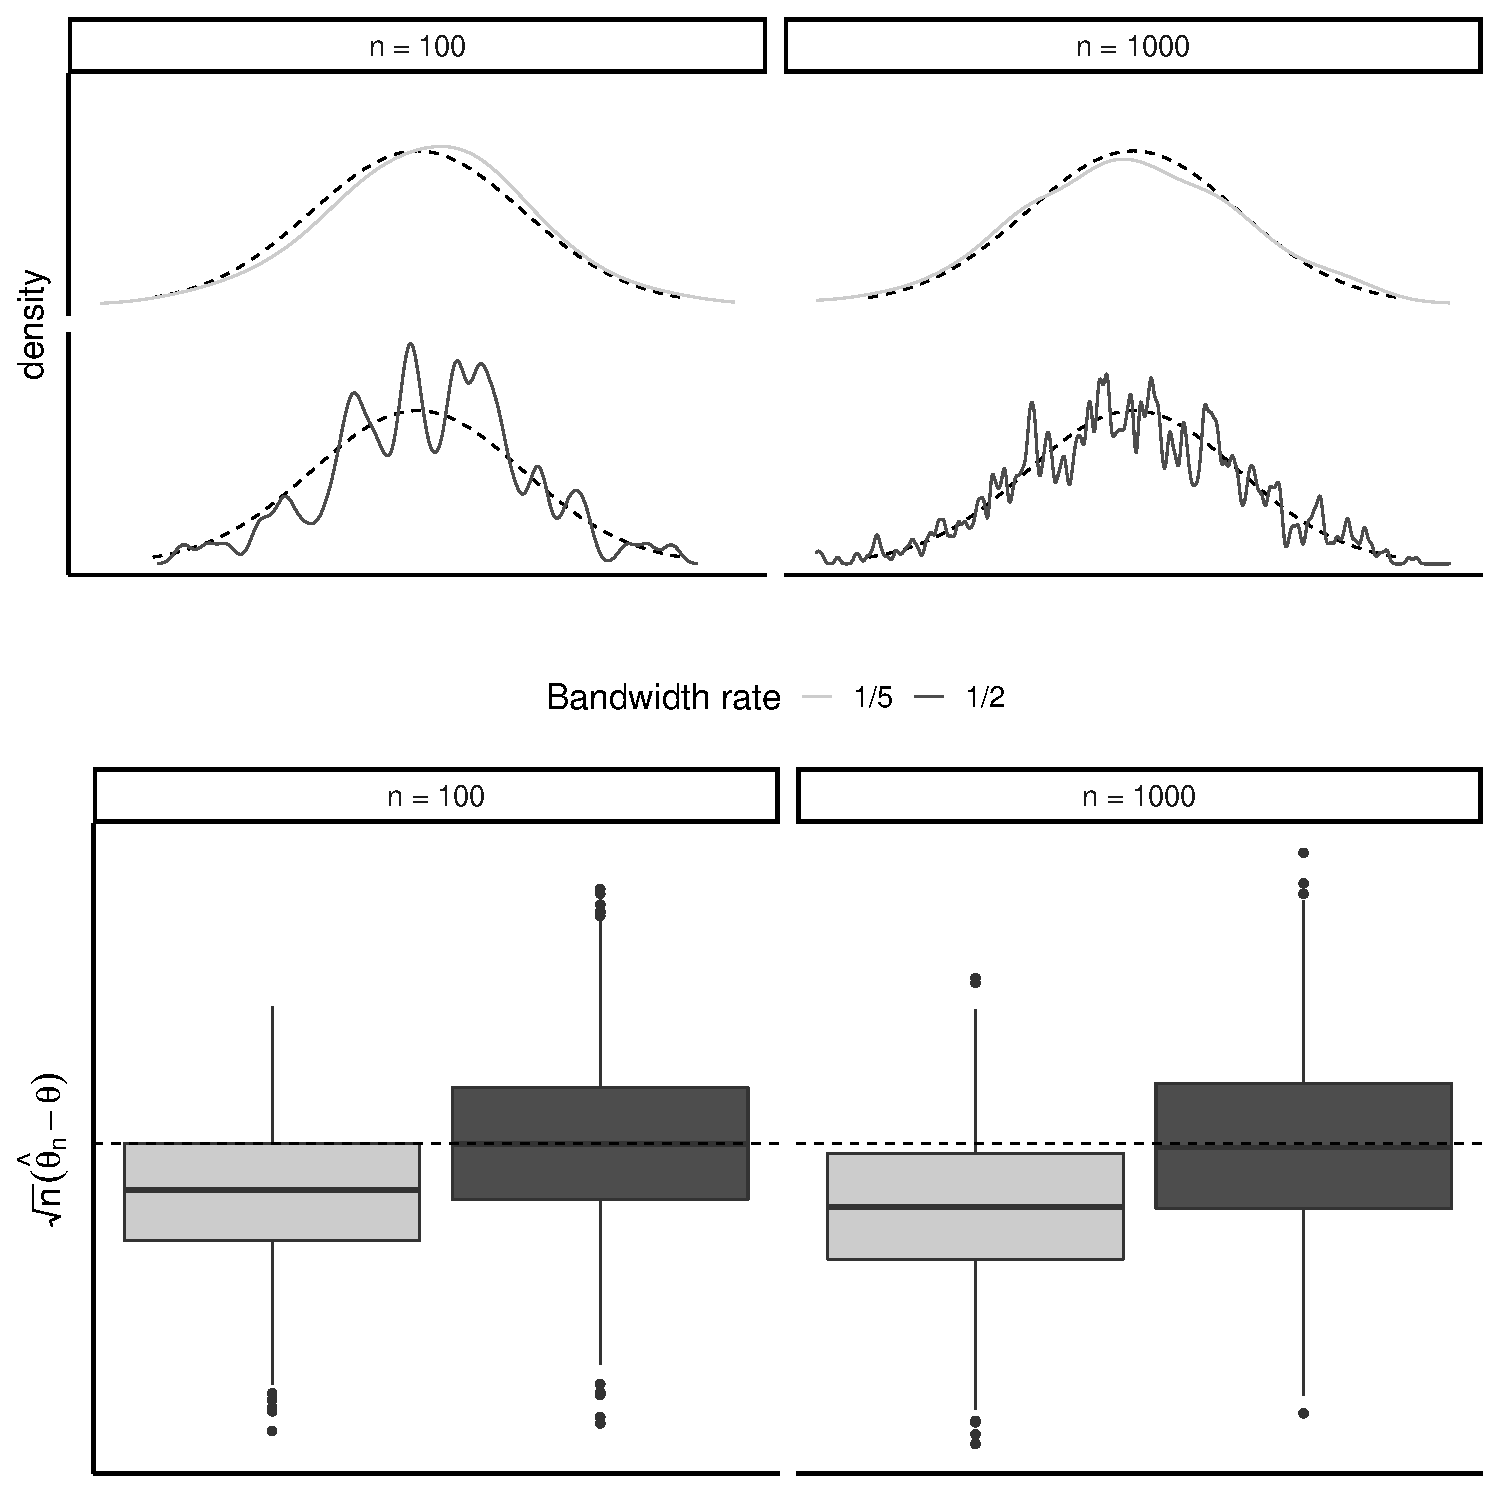
\includegraphics[width=.75\linewidth]{./figures/kernel-undersmooth-viz-presentation-3.pdf}}
    \caption{Simulation illustrating the problem for the plug-in approach. The top 2 rows give
      representative kernel density estimates for two different bandwidths scaling with $n$; the
      dashed line is the density of the distribution used to generate the data. The last row gives
      the distribution of the centralized and $\sqrt{n}$-scaled corresponding plug-in estimates
      based on 1000 Monte Carlo samples.}
    \label{fig:kernel-undersmoothed}
  \end{figure} 
\end{example}

Though the above example is somewhat silly because we already have an obvious estimator of the
parameter of interest in this situation, it clearly illustrates that the modus operandi outlined in
the two-step estimation procedure can be problematic. With this example in mind, we should not be
too confident about our ATE estimator -- in fact, with a bit more work it can be showed that similar
phenomenon happens if we use \fxnote*{todo}{the first estimator suggested above}.

The issue from example~\ref{example:kernel-cdf} can be understood more generally by considering the
decomposition
\begin{align*}
  \sqrt{n}
  \left(
  \hat{\theta}_n - \theta
  \right)
  & =  \sqrt{n}
    \left(
    \TT(\empmeas,\hat{\nu}_n) - \TT(\P,\nu)
    \right) \\
  & =
    \G{\phi( \blank, \hat{\nu}_n)}
    + \sqrt{n}
    \left\{
    \TT(\P,\hat{\nu}_n) - \TT(\P,\nu)
    \right\}
  \\
  & = \G{\phi( \blank, \hat{\nu}_n)}
    + \sqrt{n}
    \left\{
    \mathrm{D}_{\nu}{\TT}(\hat{\nu}_n - \nu)
    + \mathcal{O}_{\P}(\Vert \hat{\nu}_n - \nu \Vert^2)
    \right\}.
\end{align*}
Here we use $\mathrm{D}_{\nu}{\TT}$ to denote some kind of derivate (so be defined shortly) of the
map $\nu \mapsto \TT(\P, \nu)$, where $\P$ is held fixed, and $\Vert \blank \Vert$ is a norm defined
on the space in which the nuisance estimator $\hat{\nu}_n$ takes it values -- typically a function
space. Using empirical process theory or sample spitting, it can in many cases be shown that
$\G{\phi( \blank, \hat{\nu}_n)} = \G{\phi( \blank, \nu)} + \smallO_{\P}(1)$
\citep{van1996weak,van2000asymptotic,chernozhukov2018double}. Furthermore, if we assume that
$\hat{\nu}_n$ can be estimated at rate $n^{-1/4}$, meaning that
$\Vert \hat{\nu}_n - \nu \Vert = \smallO_{\P}(n^{-1/4})$, the decomposition becomes
\begin{equation}
  \label{eq:target-decom}
  \sqrt{n}
  \left(
    \hat{\theta}_n - \theta
  \right)
  = \G{\phi( \blank, \nu)}
  + \mathrm{D}_{\nu}{\TT}
  \left(
    \sqrt{n}(\hat{\nu}_n - \nu)
  \right)
  + \smallO_{\P}(1),
\end{equation}
where we use that a derivative $\dot{\TT}_{\nu}$ should be linear. The first term of this expression
is controlled by reference to the central limit theorem, but unless we are able to estimate $\nu$ at
the improved parametric rate of $n^{-1/2}$, we cannot hope to control the second term. Indeed, the
fact that the default kernel estimator from example~\ref{example:kernel-cdf} converges
\fxnote*{check}{at rate $n^{-2/5}$} is what ruins the asymptotic behavior of the target estimator.
In the example we showed that the target estimator could be improved by using a suitably
undersmoothed density estimator. However, we would not in general know how to choose a properly
undersmoothed nuisance estimator, so this strategy is not applicable in practice \fxnote*{ref to
  undersmoothed HAL}{(though see ...)}. If we want to use flexible machine learning estimators
(which cannot be expected to converge at parametric rate) a better strategy is to design the map to
$\TT$ such that its partial derivate $\mathrm{D}_{\nu}{\TT}$ equals 0 at $\nu$. This would make the
second term in (\ref{eq:target-decom}) vanish, and we would be able to estimate the target parameter
$\theta$ at parametric rate, while still using a nuisance estimator converging only at rate
$n^{-1/4}$.

In the next section we formally consider how to define a functional derivative, and then indicate
how this can be used to design $\TT$ with partial derivate equal to 0. In
section~\ref{sec:estim-inform-bounds} we show how these results in addition allow us to analyze and
construct \textit{efficient} estimators of $\theta$, that is, estimators with lowest possible
asymptotic variance.

\section{Functional derivatives and geometry}
\label{sec:funct-deriv-geom}

The most straightforward form of functional differentiabiliy is the generalization of the
\textit{directional derivative} of multivariate calculus. This is known as Gâteaux differentiability
and defined as follows.

\begin{definition}[Gâteaux derivate]
  Let $\mathcal{M}$ and $\mathcal{Y}$ be a normed real vector spaces,
  $\TT \colon \mathcal{M} \rightarrow \mathcal{Y}$ a map, and $x \in \mathcal{M}$ a point in the
  domain. If there exists a linear, continuous operator
  $\dot{\TT}_x \colon \mathcal{X} \rightarrow \mathcal{Y} $ such that for all $h \in \mathcal{X}$
  \begin{equation*}
    \left\Vert
      \TT(x + \epsilon h) - \TT(x) - \dot{\TT}_x(\epsilon h)
    \right\Vert_{\mathcal{Y}} = \smallO(\epsilon),
    \quad \text{when} \quad \epsilon \longrightarrow 0 \in \R,
  \end{equation*}
  we say that $\TT$ is Gâteaux differentiable at $x$. We call the operator $\dot{\TT}_x$ the
  Gâteaux derivative of $\TT$ at $x$.
\end{definition}

If the map $\TT$ is Gâteaux differentiable at $x$ then it follows from the definition that
\begin{equation}
  \label{eq:1}
    \left\Vert
      \frac{\TT(x + \epsilon h) - \TT(x)}{\epsilon} - \dot{\TT}_x(h)
    \right\Vert_{\mathcal{Y}} \longrightarrow 0,
    \quad \text{when} \quad \epsilon \longrightarrow 0.
\end{equation}
In particular, when $\mathcal{Y} = \R$ the Gâteaux derivative at $x$ in the direction $h$ can be
derived as the ordinary derivative of the real-valued function
$\epsilon \mapsto \TT(x + \epsilon h)$ evaluated at 0, i.e.,
\begin{equation}
  \label{eq:gateaux-prop}
  \dot{\TT}_x(h) = \partial_0 \TT(x + \epsilon h)
  := \frac{\partial}{\partial \epsilon} \bigg \vert_{\epsilon=0} \TT(x + \epsilon h).
\end{equation}
To simplify notation in the following we will use the notation $\partial_0f(\epsilon)$ for maps $f$
with a real domain as just defined in (\ref{eq:gateaux-prop}). Gâteaux differentiability is used by
\cite{chernozhukov2018double} to define \textit{Neyman orthogonality}: A function \fxnote*{define
  the sample space $\mathcal{Z}$}{$\phi \colon \mathcal{Z} \times \mathcal{V}\rightarrow \R$}
fulfills the Neyman orthogonality condition \fxnote*{proper def?}{(wrt.\ $\mathcal{V}$)} if the map
(as defined in section~\ref{sec:motivation})
\begin{equation*}
  F \colon \mathcal{V} \rightarrow \R, \quad \nu \longmapsto F(\nu) :=\P[\phi(Z, \nu)]
\end{equation*}
is Gâteaux differentiable at $\nu$ with vanishing derivative, i.e., $\dot{F}_{\nu}(h) = 0$ for all
$h \in \mathcal{V}$.

Neyman orthogonality ensures that the second component of the decomposition in
(\ref{eq:target-decom}) vanishes, and as the condition can be checked using (\ref{eq:gateaux-prop})
it is rather straightforward to verify that a given function fulfills the condition. Still, Gâteaux
is a weak form of differentiability; for instance, as it is equivalent to the directional derivative
for ordinary multivariate functions, Gâteaux differentiability is not enough to guarantee (ordinary)
differentiability of such functions. Similarly, to get a richer theory in the functional setting a
stronger notion of differentiability is needed. For our setting, a particular useful concept is
\textit{Hadamard} differentiability.

\begin{definition}[Hadamard derivate]
  \label{def:hadamard-diff}
  Let $\mathcal{M}$ and $\mathcal{Y}$ be a normed real vector spaces,
  $\TT \colon \mathcal{M} \rightarrow \mathcal{Y}$ a map, and $x \in \mathcal{M}$ a point in the
  domain. If there exists a linear, continuous operator
  $\dot{\TT}_x \colon \mathcal{X} \rightarrow \mathcal{Y} $ such that
  \begin{equation*}
    \left\Vert
      \frac{\TT(x + \epsilon_n h_n) - \TT(x)}{\epsilon_n} - \dot{\TT}_x(h)
    \right\Vert_{\mathcal{Y}} \longrightarrow 0,
  \end{equation*}
  for any $\epsilon_n \rightarrow 0$ and $\{h_n\}_{n \in \N} \subset \mathcal{X}$ with
  $h_n \rightarrow h \in \mathcal{X}$, we say that $\TT$ is Hadamard differentiable at $x$ and call
  the operator $\dot{\TT}_x$ the Hadamard derivative of $\TT$ at $x$.
\end{definition}

Comparing this definition with (\ref{eq:1}) we see that the only difference is that the linear
approximation provided by $\dot{\TT}_x$ should holds along any \textit{converging sequence} $h_n$
and not merely in a fixed direction $h$. For this reason Hadamard differentiability is also known a
\textit{path-wise} differentiability. A still stronger condition is to demand that the approximation
should hold for any \textit{bounded sequence} $h_n$; this gives the concept of \textit{Fréchet}
differentiability, which we will not use in this text. One can show that \textit{if} a map is
Hadamard (or Fréchet) differentiable, then the Hadamard (or Fréchet) derivative is equal to the
Gâteaux derivative. Hence, to find the Hadamard derivative of a given functional $\TT$, the common
strategy is to first use high school math tools to calculate (\ref{eq:gateaux-prop}) and then verify
that the obtained candidate fulfills the requirements of definition~\ref{def:hadamard-diff}.

So far we have assumed the domain to be a \textit{linear} space. When working with probability
measures, this is often not the case, and hence we need one final definition, which allows the
operator $\TT$ and its derivative $\dot{\TT}$ to be defined only on subsets of the normed vector
space $\mathcal{M}$. We should think of the following as mirroring differentiation of a multivariate
function defined on a manifold embedded in a higher dimensional Euclidean space (for instance, a
surface embedded in $\R^3$, \fxnote*{Make the picture}{see picture}).

\begin{definition}[Tangential Hadamard derivative]
  Let $\mathcal{P}$ and $\dot{\mathcal{P}}_x$ be subsets of the normed real vector space
  $\mathcal{M}$, with $x \in \mathcal{P} \subset \mathcal{M}$. For a map
  $\TT \colon \mathcal{P} \rightarrow \mathcal{Y}$, we say that $\TT$ is \textit{Hadamard
    differentiable (at $x$) tangential to $\dot{\mathcal{P}}_x$} if there exists a continuous,
  linear operator $\dot{\TT}_x \colon \dot{\mathcal{P}}_x \rightarrow \mathcal{Y}$ such that
  \begin{equation*}
    \left\Vert
      \frac{\TT(x + \epsilon_n h_n) - \TT(x)}{\epsilon_n} - \dot{\TT}_x(h)
    \right\Vert_{\mathcal{Y}} \longrightarrow 0, 
  \end{equation*}
  for any $\{h_n\} \subset \mathcal{M}$ and $\{\epsilon_n\} \subset \R$ with
  $h_n \rightarrow h \in \dot{\mathcal{P}}_x$, $\epsilon_n\rightarrow 0$, and
  $x + \epsilon_n h_n \in \mathcal{P}$.
\end{definition}

The only change from the previous definition is that the ``path'' $x + \epsilon_n h_n$ is restricted
to lie in the subset $\mathcal{P}$, and that the ``direction'' is $h$ is restricted to lie in
$\dot{\mathcal{P}}_x$.

Finally, to be able to talk about differentiability of the statistical problem \fxnote*{define this
  earlier}{$(\mathcal{P}, \TT)$}, we need to embed the model $\mathcal{P}$ into a suitable normed
vector space. To do so we now assume for simplicity that the family $\mathcal{P}$ is dominated by a
single $\sigma$-finite measure $\mu$ (for our running example of the ATE this measure would be a
product of Lebesgue and counting measures), and then think of $\mathcal{P}$ as lying inside the
Banach space $\mathcal{M}_{\mu}$ of finite signed measures dominated by $\mu$ equipped with the
variational norm
\begin{equation*}
  \Vert M \Vert_{\mathcal{M}_{\mu}} = \int |m |\diff \mu, \quad \text{ for } \quad M = m \cdot \mu.
\end{equation*}

% We can then represent every element $\P \in \mathcal{P}$
% as an element in the space of quadratically $\mu$-integrable functions, $\mathcal{L}^2_{\mu}$,
% through the map
% \begin{equation}
%   \label{eq:iso-map}
%   \mathcal{P} \ni \P \longmapsto s(\P) := \sqrt{p} \in \mathcal{L}^2_{\mu},
%   \quad \text{for} \quad \P = p\cdot\mu.
% \end{equation}
% By the Jordan-Hahn decomposition the map $s$ can be extended to \fxnote*{I think this is
%   correct...?}{a bijection between $\mathcal{L}^2_{\mu}$ and the space of finite signed measures
%   dominated by $\mu$}, which we denote as $\mathcal{M}_{\mu}$. If we let $\mathcal{M}_{\mu}$ inherit
% the vector space and Hilbert space structure from $\mathcal{L}_{\mu}^2$,\footnote{Here we mean that
%   we should, for instance, define addition of $M_1$ and $M_2$ in $\mathcal{M}_{\mu}$ as
%   $s^{-1}(s(M_1) + s(M_2))$, and $\langle M_1, M_2 \rangle_{\mathcal{M}_{\mu}}$ as
%   $\langle s(M_1), s(M_2) \rangle_{\mathcal{L}_{\mu}^2}$, and so on.} we have an isomorphism between
% these two spaces; hence, we can either think of $\mathcal{P}$ as embedded into the space of finite
% signed measure $\mathcal{M}_{\mu}$, or as being represented by their square-root densities in
% $\mathcal{L}_{\mu}^2$. The metric introduced on $\mathcal{M}_{\mu}$ in this way is the (extended)
% Hellinger distance \citep{bickel1993efficient,steerneman1983total}, but due to the non-linearity of
% $s$, the last representation is more useful for doing actual calculations. We assume in the
% following that $\mathcal{M}_{\mu}$ is equipped with norm and vector space structure inherited from
% $\mathcal{L}_{\mu}^2$ through $s$ defined in (\ref{eq:iso-map}).

\begin{definition}[Tangent space for $\mathcal{P}$]
  Let $\mathcal{P} \subset \mathcal{M}_{\mu}$ be a collection of probability measures and let
  $\P \in \mathcal{P}$. For any one-dimensional path
  $\epsilon \mapsto \P_{\epsilon} \in \mathcal{P}$ with $\P_0 =\P$, which is Hadamard\footnote{When
    the domain is $\R$, all the previously considered types of differentiability are equivalent, so
    any type could be used here.} differentiable at 0, let $\partial_0\P_{\epsilon}$ be the
  derivative, and let $\{\partial_0\P_{\epsilon}\}$ be the collection of derivatives of all such paths. We call
  the \fxnote*{should there be added some note about this -- always sensible thing, or need to
    assume something?}{closed linear span} of this collection the \textit{tangent space of
    $\mathcal{P}$ at $\P$} and denote it by $\dot{\mathcal{P}}_{\P}$. Formally,
  \begin{equation*}
    \dot{\mathcal{P}}_{\P}
    := \overline{\mathrm{span}}
    % {\dot{\mathcal{P}}_{\P}^0} , \quad 
    % \dot{\mathcal{P}}_{\P}^0    :=
    % \left\{ \frac{\diff}{\diff \epsilon } \Big\vert_{\epsilon=0} \P_{\epsilon}
    \left\{ \partial_0\P_{\epsilon}
      \midd \epsilon \mapsto \P_{\epsilon} \text{ is Hadamard differentiable and } \P_0 = \P  \right\}.
  \end{equation*}
\end{definition}

The definition of a tangent space for a collection of probability measures simple mimics the
definition of a tangent space for a surface embedded in $\R^3$: We move along differentiable paths
through a given point on the surface, and the tangent space is then the span of the derivatives of
all such paths. With a differentiable structure on the collection $\mathcal{P}$ we can talk about a
\textit{gradient} of a functional defined on this set.

\begin{definition}[Canonical gradient]
  Let $(\mathcal{P}, \TT)$ be a \fxnote*{}{statistical problem}, with
  $\mathcal{P} \subset \mathcal{M}_{\mu}$, and $\dot{\mathcal{P}}_{\P}$ the tangent space of
  $\mathcal{P}$ at $\P \in \mathcal{P}$. If $\TT \colon \mathcal{P} \rightarrow \R$ is Hadamard
  differentiable at $\P$ tangential to $\dot{\mathcal{P}}_{\P}$, we refer to the Hadamard derivative
  $\dot{\TT}_{\P}$ as the \textit{canonical gradient of the statistical problem}.
\end{definition}

% \subsection{Representations of tangent spaces and canonical gradients}
% \label{sec:repr-tang-space}

The definitions of the tangent space $\dot{\mathcal{P}}_{\P}$ and the gradient $\dot{\TT}_{\P}$
above capture the intuitive meaning of these concepts as generalizations of well-known concepts from
multivariate calculus: The statistical model $\mathcal{P}$ is viewed as a subset of the unit sphere
in $\mathcal{M}_{\mu}$ and the canonical gradient $\dot{\TT}_{\P}$ is simply the
infinite-dimensional version of the gradient of a map defined on a surface in Euclidean space. We
shall see in a moment why this object $\dot{\TT}_{\P}$ is of interest for the statistician, but
firstly we consider a different representation of $\mathcal{P}$ which allows us to represent
$\dot{\mathcal{P}}_{\P}$ as a subset of $\lp$; this is particularly useful as we then
have the rich Hilbert space structure of $\lp$ at our disposal.

For a fixed element $\P \in \mathcal{P}$ with $\mu$-density $p$, consider a one-dimensional
parametric submodel of $\mu$-densities $p_{\epsilon}$ with $p_0=p$ and
$p_{\epsilon} \cdot \mu \in \mathcal{P}$ for \fxnote*{interval...}{all $\epsilon$}. Restricting
attention to such submodels for which the function
\begin{equation*}
  \dot{\ell}_0 = \partial_0 \log(p_{\epsilon})
\end{equation*}
exists as an element in $\lp$, we call $\dot{\ell}_0$ the \textit{score} of the
submodel $p_{\epsilon}$. This reflects the terminology used in likelihood inference for ordinary
parametric models.

\begin{proposition}
  \label{prop:repr-tang-spac}
  The tangent space $\dot{\mathcal{P}}_{\P}$ \fxnote*{right words to use? More precise...?}{can be
    represented as} the closed linear span of all score functions as defined above, considered as a
  subset of $\lp$, which we denote as
  $\Gamma_{\P} := \overline{\mathrm{span}}\{\dot{\ell}_0\} \subset \lp$.
\end{proposition}

\begin{proof}
  \fxnote*{todo/finish. Pretty sure this results is correct...}{Something like this:} We can also
  represent $\mathcal{P}$ as a subset of $\mathcal{L}_{\mu}^2$ through the map
  $\P \mapsto \sqrt{p}$, and the topology on $\mathcal{P}$ induced in this way is \fxnote*{check --
    also the generalized versions on the whole space?}{the same as that induced} by
  $\Vert \blank \Vert_{\mathcal{M}_{\mu}}$ \citep{bickel1993efficient}. This implies that
  convergence of $(\P_{\epsilon h} - \P_{0})\epsilon^{-1}$ in $\mathcal{M}_{\mu}$ is equivalent to
  convergence of convergence of $(\sqrt{p_{\epsilon h}} - \sqrt{p_{0}})\epsilon^{-1}$ in
  $\mathcal{L}_{\mu}^2$. \fxnote*{finish}{Then Gâteaux + map with $/p_0$...}
\end{proof}

Proposition~\ref{prop:repr-tang-spac} in essence states that we can think of the tangent space as
the (closed linear span of) the collection of score functions for all parametric submodels
$\mathcal{P}_{\epsilon}$ passing through $\P$; hence we shall often simply identify
$\dot{\mathcal{P}}_{\P}$ with $\Gamma_{\P}$. This representation in turn implies the following
useful representation of the canonical gradient.

\begin{proposition}
  \label{prop:repr-can-gradient}
  Let $(\mathcal{P}, \TT)$ be a statistical problem with canonical gradient
  $\dot{\mathcal{\TT}}_{\P}$ at $\P \in \mathcal{P}$. There exists a unique element
  $\phi_{\P} \in \Gamma_{\P}$ such that
  \begin{equation}
    \label{eq:2}
    \partial_0 \TT(\P_{\epsilon})
    = \langle \phi_{\P}, \dot{\ell}_0 \rangle_{\P}
    % =  \int \phi \dot{\ell}_0  \diff \P,
  \end{equation}
  holds for any differentiable submodel $\P_{\epsilon}$ with score function $\dot{\ell}_0$.
\end{proposition}

\begin{proof}
  The \fxnote*{introduce or mention before}{chain rule for Hadamard derivative} implies that
  $\partial_0 \TT(\P_{\epsilon}) = \dot{\TT}_{\P}(\partial_0 \P_{\epsilon})$, and then the
  representation given by proposition~\ref{prop:repr-tang-spac} implies that this expression equals
  $\Phi_{\P}(\dot{\ell}_0)$ for some continuous linear functional
  $\Phi_{\P} \colon \Gamma_{\P} \rightarrow \R$. As $\Gamma_{\P}$ is a closed subspace of a Hilbert
  space it is itself a Hilbert space, and hence Riesz representation theorem (for Hilbert spaces)
  gives the existence of a unique element $\phi_{\P} \in \Gamma_{\P}$ such that
  $\Phi_{\P}(\dot{\ell}_0) = \langle\phi_{\P}, \dot{\ell}_0\rangle$ for all elements
  $\dot{\ell}_0 \in \Gamma_{\P}$.
\end{proof}

By the chain rule of ordinary multivariate calculus we have for a differentiable function
$f\colon\R^d \rightarrow \R$ and any smooth curve $s\colon\R\rightarrow \R^d$ with
$s(0) = x_0 \in \R^d$ that
\begin{equation*}
  \partial_{0} (f\circ s) = \nabla f(s(0)) \cdot (\partial_{0}s )^{\T}
  =
  \left\langle
    \nabla f(x_0) ,  \partial_{t}s 
  \right\rangle,
\end{equation*}
and as $\R^d$ can be spanned by smooth 1-dimensional curves, this property characterizes the
gradient locally. Proposition~\ref{prop:repr-can-gradient} above states that this characterization
extends to the Hilbert space setting with Hadamard differentiability, and in fact this
characterization \fxnote*{I think this is correct}{can be used to define} Hadamard differentiability
of the map $\TT$ tangential to $\Gamma_{\P}$ \citep[A.5]{bickel1993efficient}.

As with the identification $\dot{\mathcal{P}}_{\P}= \Gamma_{\P}$ we also \fxnote*{}{identify} the
function $\phi_{\P}$ with the canonical gradient $\dot{\Psi}_{\P}$. Note that if $\Gamma_{\P}$ is a
proper subset of $\lp$ there can be several functions $\tilde{\phi} \in \lp$ fulfilling condition
(\ref{eq:2}); we refer to such functions as \textit{gradients}. It follows from standard Hilbert
space theory that the unique canonical gradient $\phi_{\P}$ can be derived from any gradient
$\tilde{\phi}$ as the projection onto $\Gamma_{\P}$, i.e.,
$ \phi_{\P} = \Pi(\tilde{\phi} \mid \Gamma_{\P})$. This geometric representation of the tangent
space and the gradient is very useful.

Returning to the decomposition in (\ref{eq:target-decom}) we have the following results.

\begin{proposition}
  Let $(\mathcal{P}, \TT)$ be a statistical problem with $\mathcal{P}$ dominated by $\mu$ and such
  that $\TT(\P) = \P[\phi(Z, \nu(\P))]$ for some function
  $\phi\colon \mathcal{Z} \times \mathcal{V} \rightarrow \R$. If $\phi(\blank, \nu(\P))$ is the
  canonical gradient of $(\mathcal{P}, \TT)$ then, \fxnote*{can these be made precise?}{under
    regularity conditions}, $\phi$ fulfills the Neyman orthogonality condition \fxnote*{ok? Or
    should it actually be $\nu(\mathcal{P})$?}{(wrt.\ $\dot{\nu}_{\P}(\dot{\mathcal{P}}_{\P})$)},
  \fxnote*{some unaligned defintions here?}{i.e.},
  $\partial_0 \P[\phi(\blank, \nu(\P) + \epsilon h)] = 0$ for all
  $h \in \dot{\nu}_{\P}(\dot{\mathcal{P}}_{\P})$.
\end{proposition}

\begin{proof}
  Under regularity conditions that allow us to interchange integration and differentation in the
  following, we have for any \fxnote*{}{differentiable} path
  $\{\P_{\epsilon}\}_{\epsilon} \subset \mathcal{P}$ with $\P_0=\P$ that
  \begin{align}
    \label{eq:3}
    \begin{split}
      \partial_0 \TT(\P_{\epsilon})% = \partial_0 \P_{\epsilon}[\phi(Z, \nu(\P_{\epsilon}))]
      & =\partial_0 \int p_{\epsilon}(z) \phi(z, \nu(\P_{\epsilon})) \diff \mu(z) \\
      & = \int p \{\partial_0  \phi(z, \nu(\P_{\epsilon}))\} +  \{\partial_0 p_{\epsilon}(z)\} \phi(z, \nu(\P)) \diff \mu(z) \\
      & = \partial_0 \P[ \phi(\blank, \nu(\P_{\epsilon}))] +
      % \P[\partial_0\log p_{\epsilon} \, \phi(\blank, \nu(\P))].
      \langle \dot{\ell}_0, \phi(\blank, \nu(\P))\rangle_{\P},
    \end{split}
  \end{align}
  where $\dot{\ell}_0$ is the score function of the parametric submodel $\P_{\epsilon}$ and we used
  the relation $\partial_{0}\log p_{\epsilon} = (\partial_{0} p_{\epsilon})p_0^{-1}$. As
  $\phi(\blank, \nu(\P))$ is the canonical gradient at $\P$,
  proposition~\ref{prop:repr-can-gradient} and (\ref{eq:3}) imply that
  $\partial_0 \P[ \phi(\blank, \nu(\P_{\epsilon}))]=0$. \fxnote*{finish the argument with something
    like this}{Assuming Hadamard differentiability of $\P \mapsto \nu(\P)$ and
    $\nu \mapsto F(\nu) = \P[\phi(\blank, \nu)]$ we can write
    $\partial_0 \P[\phi(\blank, \nu(\P) + \epsilon h)] = \partial_0 \dot{F}_{\nu(\P)}(h)$, for
    $h\in\dot{\nu}_{\P}(\dot{\mathcal{P}}_{\P})$; hence (by definition of $\dot{\mathcal{P}}_{\P}$)
    we can find path $\P_{\epsilon}$ such that $\dot{\nu}_{\P}(\partial_0 \P_{\epsilon}) = h$, and
    then picking this path in the expression above we get $\partial_0 \dot{F}_{\nu(\P)}(h) =0$.}
\end{proof}

The result shows that estimators based on the canonical gradient has a ``build-in'' so-called
\textit{debiasing} mechanism because the first order bias (the second expression in
(\ref{eq:target-decom})), due to estimation of the nuisance parameter $\hat{\nu}_n$, vanishes. This
debiasing mechanism is crucial for $n^{-1/2}$-rate inference of a target parameter in a statistical
model with nuisance parameters that are not estimable at this rate themselves. \fxnote*{What is the
  intuitive explanation of this result? In standard calculus, the derivatives are orthogonal -- can
  this intuition explain the results?}{}

Note that the fact that a function $\phi$ fulfills the Neyman orthogonality condition does not
necessarily imply that $\phi$ is the canonical gradient (see, for instance,
\cite{chernozhukov2016double} for an example). This can be seen from the fact that we in the proof
above only used that $\phi(\blank, \nu(\P))$ satisfies (\ref{eq:2}), and not that
$\phi(\blank, \nu(\P)) \in \Gamma_{\P}$; hence, \fxnote*{I think this must be correct}{any gradient
  for the statistical problem will fulfill the Neyman orthogonality condition} (under regularity
conditions).

\section{Estimators and information bounds}
\label{sec:estim-inform-bounds}

The last result of the previous section demonstrated that estimators based on the canonical gradient
provide target parameter estimators with no first order bias. In this section we show that they also
provide \textit{efficient} estimators. 

\fxnote*{briefly to this}{
  \begin{itemize}
  \item RAL estimators and IFs
  \item Information bounds
  \item Connection to canonical gradient
  \end{itemize}
}

\bibliography{./latex-settings/default-bib.bib}

\end{document}